\section{Results}
Many nice figures
\begin{enumerate}
	\item Histograms
	\item Histograms 3 directions
	\item PC
\end{enumerate}

\subsection{Activation Distribution on a  Fixed Force Vector}

\begin{figure}[ht]
   \begin{center}
    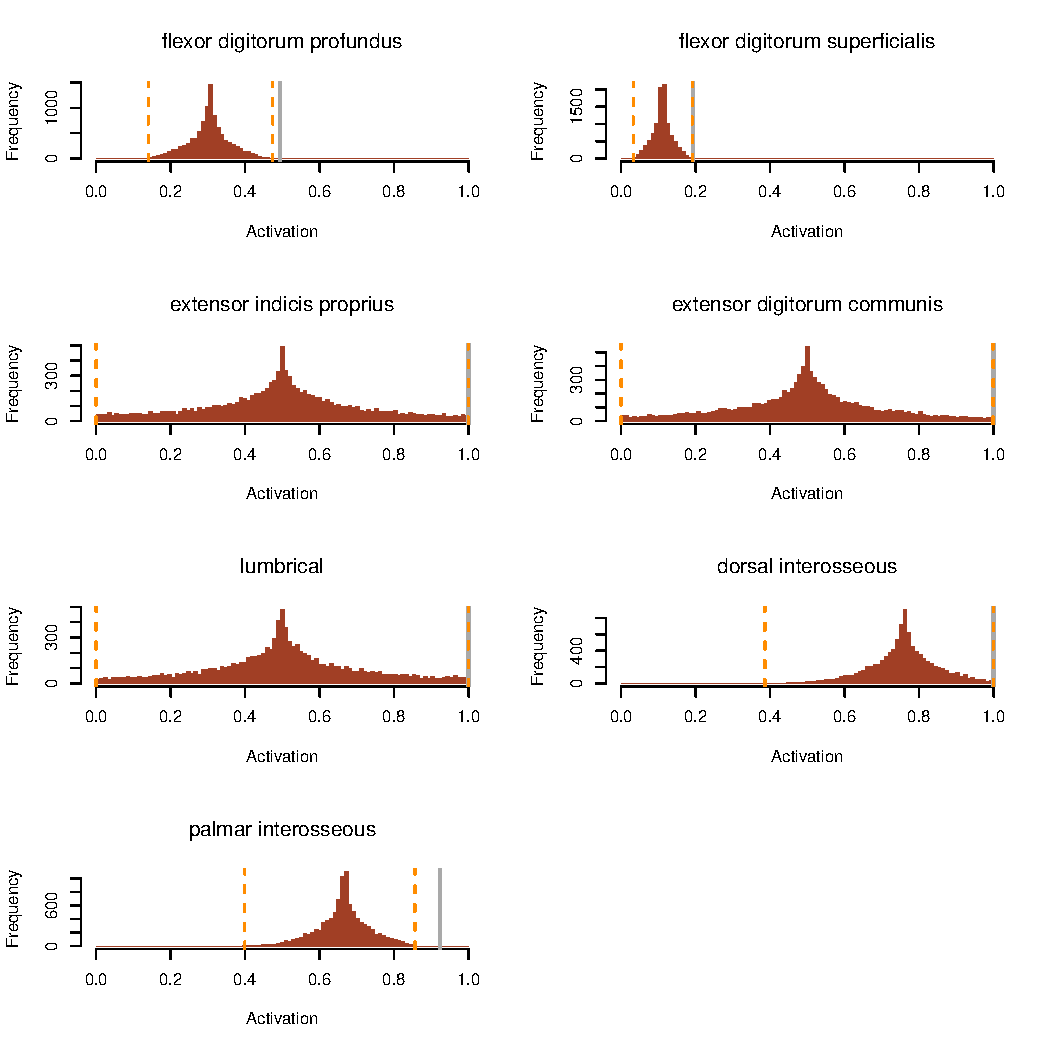
\includegraphics[width=0.5\textwidth]{figs/raw_histograms.pdf}
  \end{center}
  \caption{Histogram for Fixed Force}
  \label{fig_rawhisto}
\end{figure}
Feasible activations for palmar submaximal force production (at X\percent) suggest very similar solution distributions across mslces 3,4,5. Also, they are not bounded by the task in activation; for each of these muscles, their activation can be maximal or zero, and the model finger can still generate the force.

All of the muscles have a central peak between the bounds, suggesting that the activation space is not skewed, but is rather a broad shape. The peak refers to the slice of the activation space where the highest number of solutions exist. Said another way, the integral of that slice represents the solutionspace volume.




\subsection{Changing Output Force in 3 Directions}
We discuss different forces into three different directions, which are given by the palmar direction ($x$-direction), the distal direction ($y$-direction) and the sum of them. The maximal forces into each direction are given by ??, ?? and ?? respectively. For $\alpha = 0.1, 0.2, \dots, 0.9$, we give the histograms where the force is $\alpha \cdot F_{\max}$, where $F_{\max}$ is the maxium output force in the corresponding direction. 

\begin{figure}[ht]
   \begin{center}
    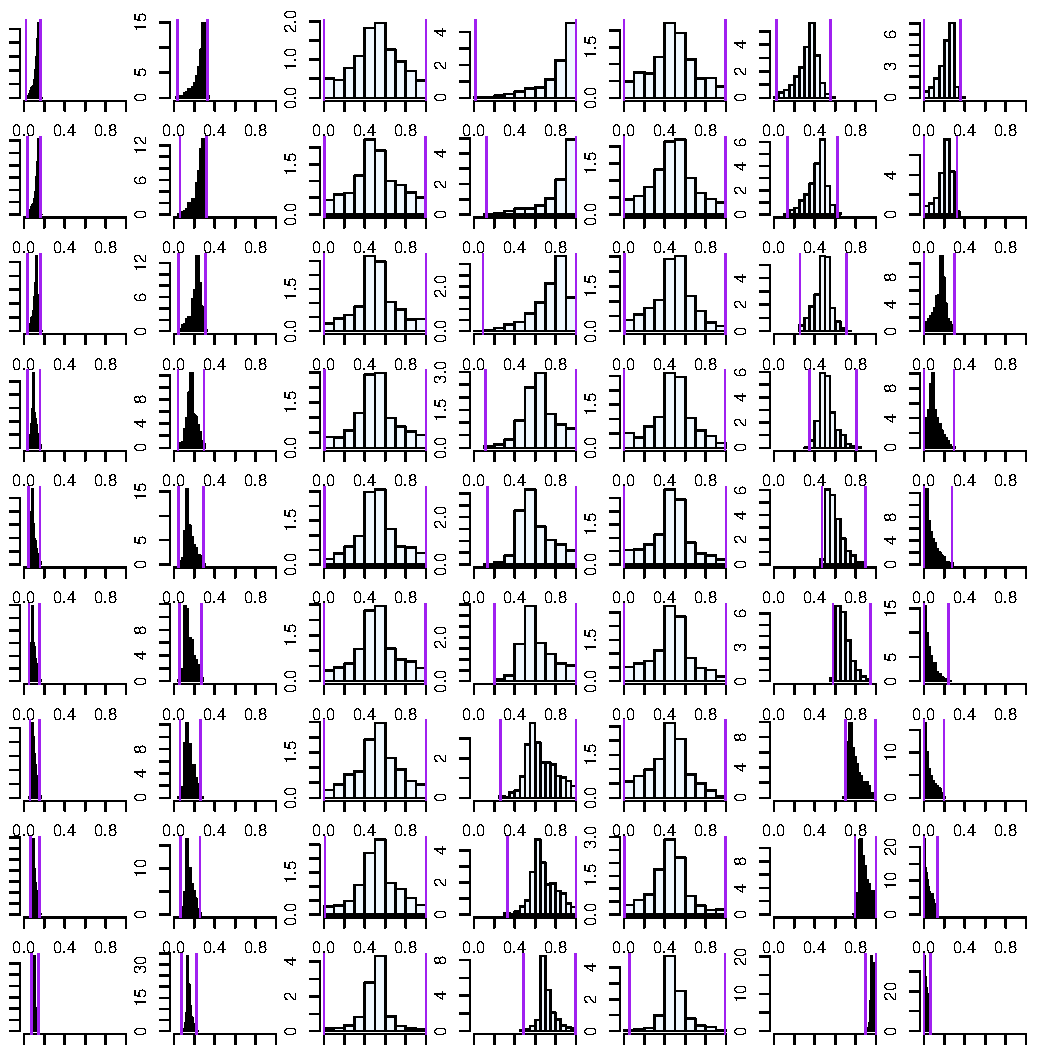
\includegraphics[width=1.0\textwidth]{XalphaProgression.pdf}
  \end{center}
  \caption{Histogram for $x$-Direction}
  \label{fig_xhisto}
\end{figure}


\begin{figure}[ht]
   \begin{center}
    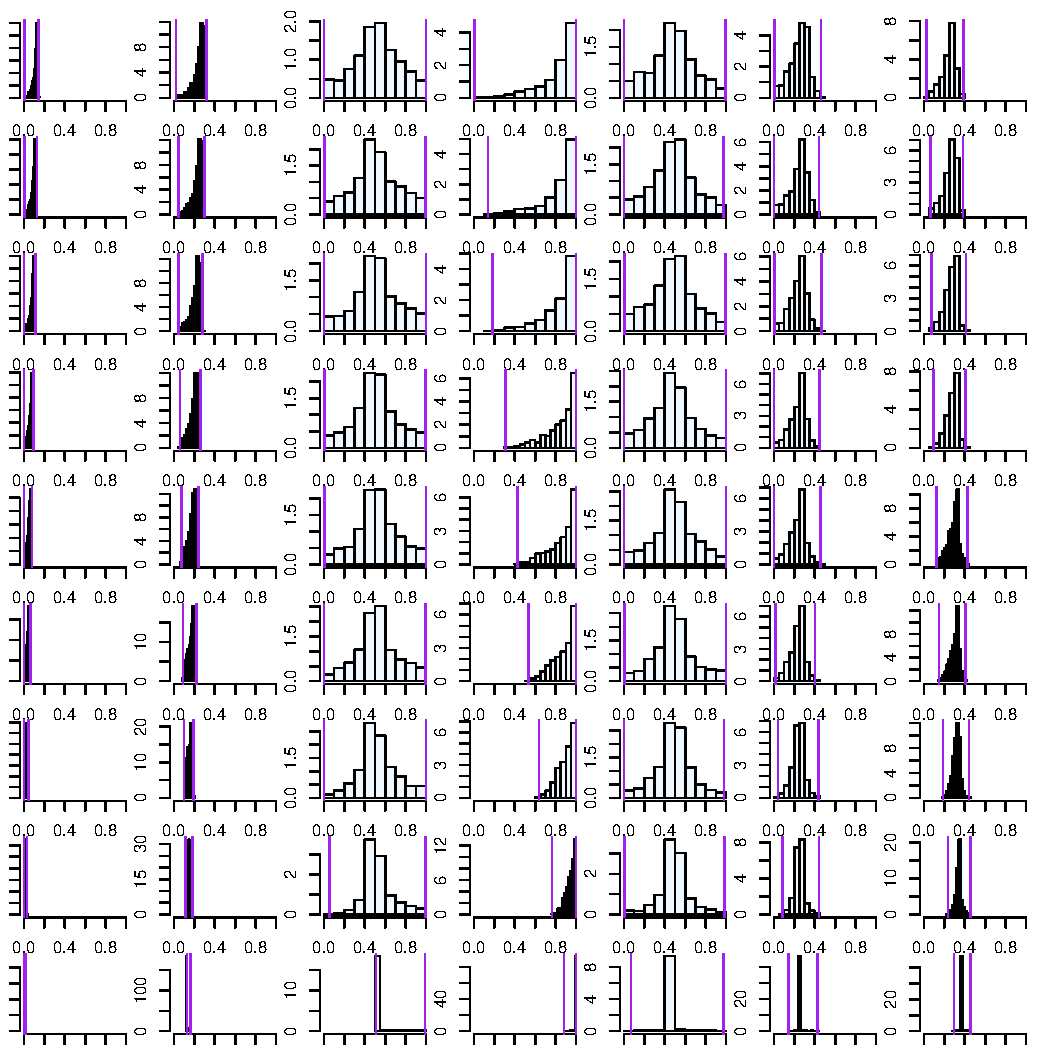
\includegraphics[width=1.0\textwidth]{YalphaProgression.pdf}
  \end{center}
  \caption{Histogram for $xy$-Direction}
  \label{fig_yhisto}
\end{figure}

\begin{comment}
\begin{figure}[ht]
   \begin{center}
    \includegraphics[width=1.0\textwidth]{XYalphaProgression.pdf}
  \end{center}
  \caption{Histogram for $xy$-Direction}
  \label{fig_xyhisto}
\end{figure}
\end{comment}

\subsection{Parallel Coordinates}
The relationship between the histograms shown above, and the parallel coordinate interactive plots, is the measure of density across each muscle. Peak density areas of the histogram will appear as dark blue sections of the muscle histograms, as those regions are host to more solutions.

Although we computed XXX solutions for each level of alpha, we generate 1000 feasible solution points. Although using higher numbers of points works in the parallell coordinates system, we elected to reduce sample size to provide realtime response rates for interactive constraining of muscles and cost functions.


Typically, selecting solutions where one muscle is constrained to be lower activation results in one or multiple compensatory increases in activation for the other muscles; this is apparent when the bulk of the solutions moves up while constraining one muscle down. When we see many solution lines in parallel across two muscles, it suggests a consistent relationship between the two. Consistent slopes between the solutions suggest an antagonist relationship. When the slope appears close to zero, the two muscles are equal in effect in their angaonistic relationship; a negative slope suggests the first muscle is less influential in task generation, while a positive slope suggests higher influence.

When two muscles have highly mixed slopes, it could suggest that these muscles do not have a geometric interdependency, and could have orthogonal contributions to output force. 

\begin{figure}[ht]
   \begin{center}
    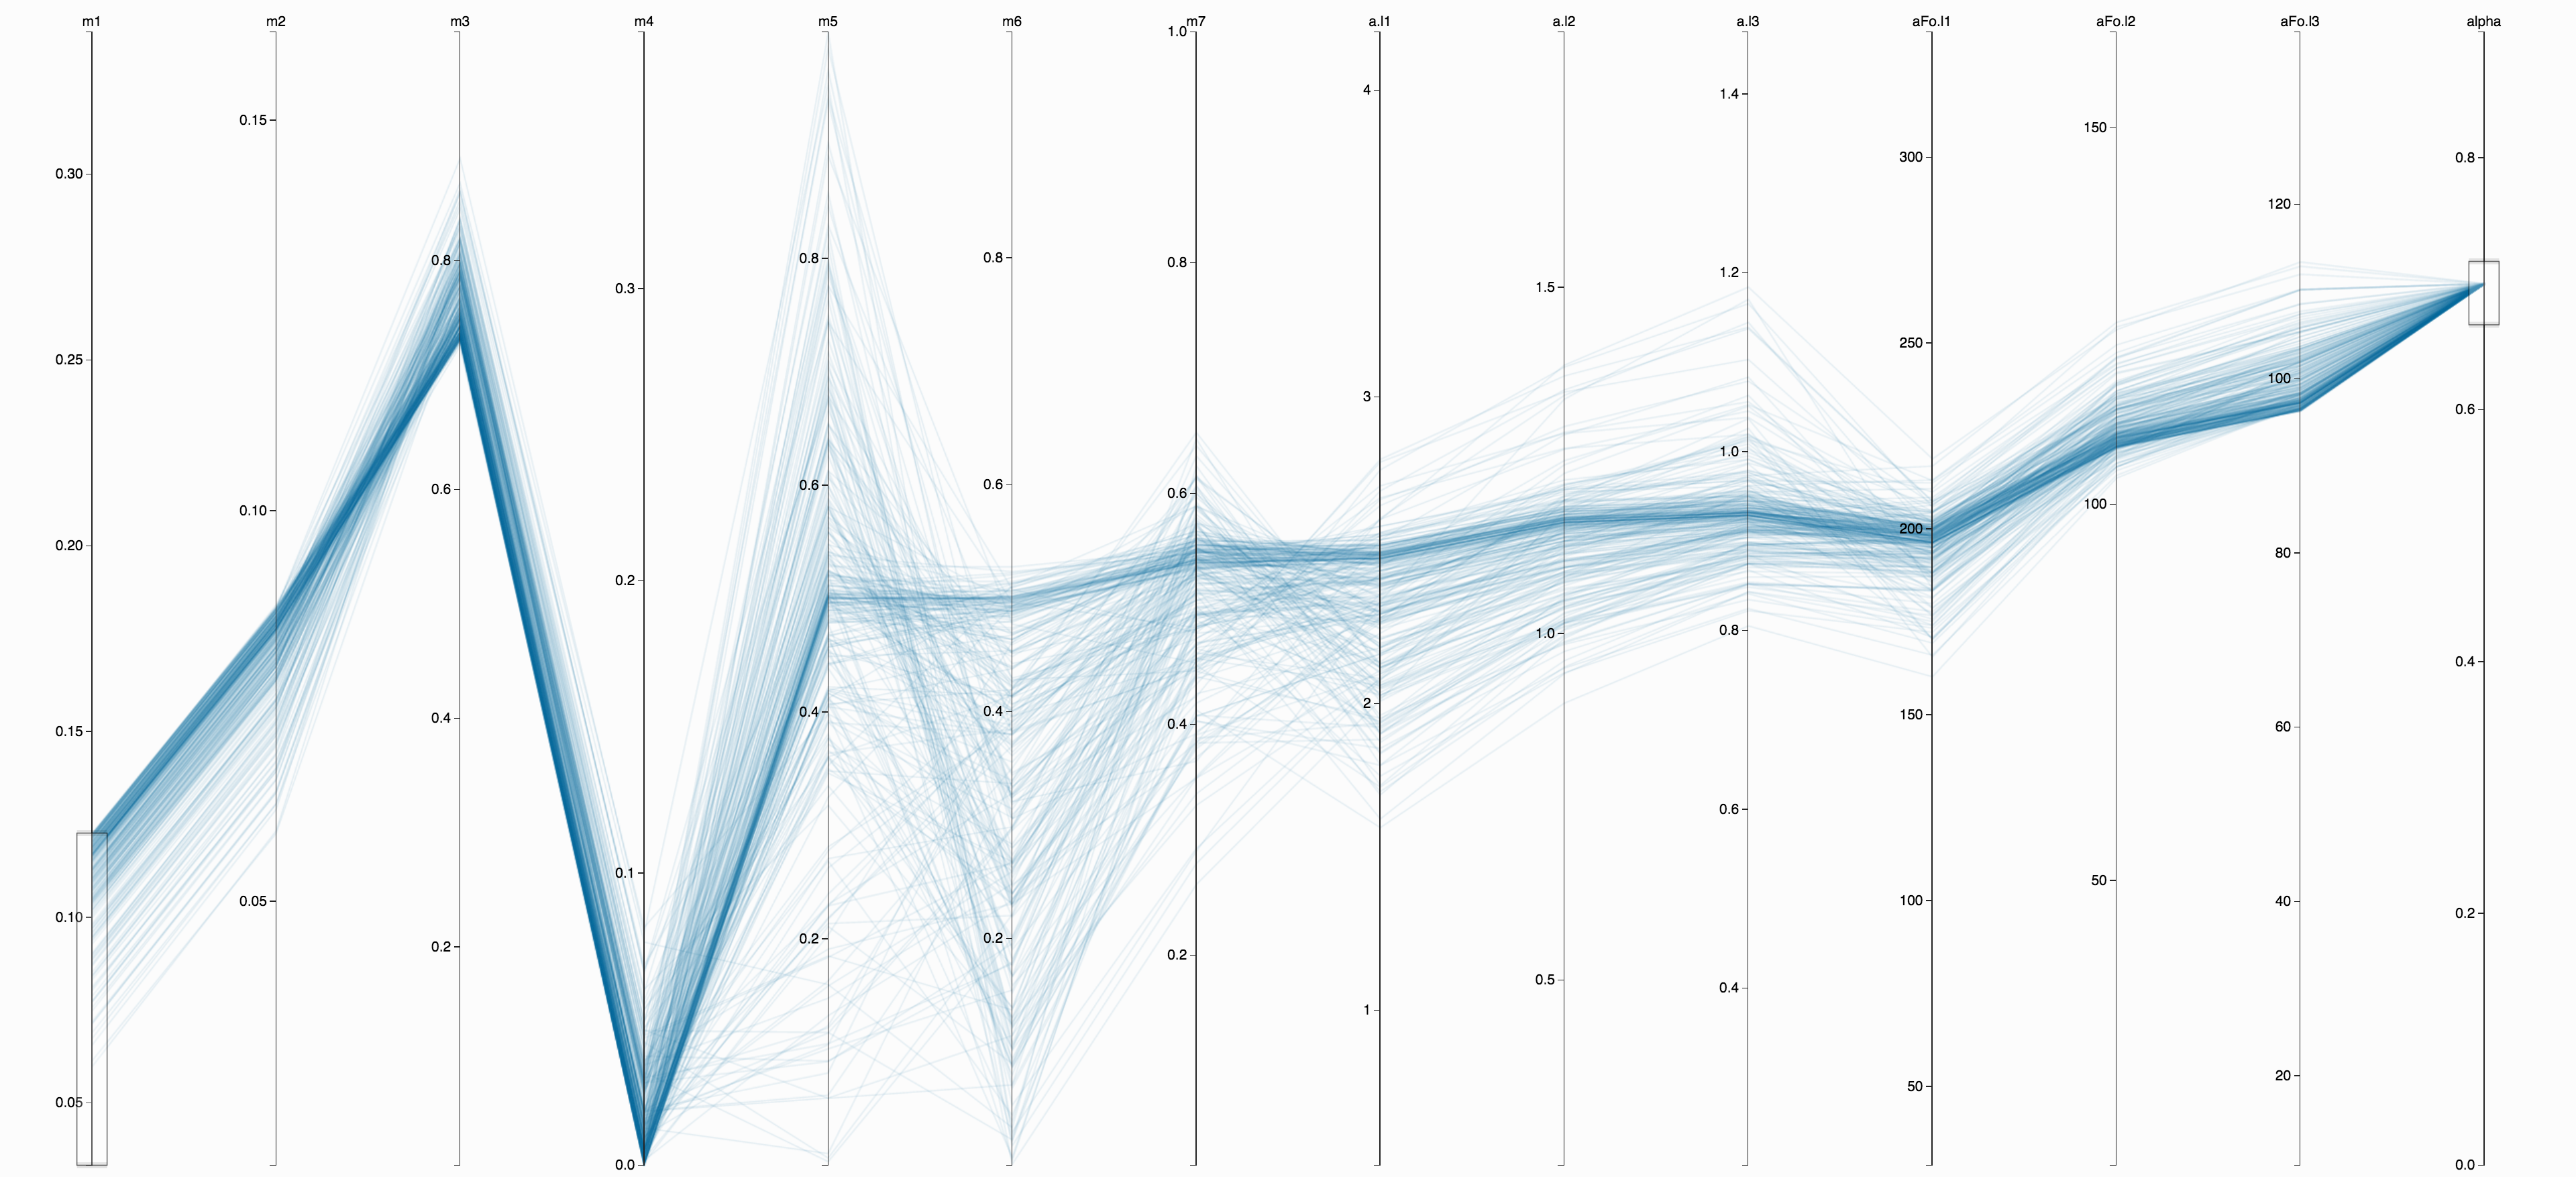
\includegraphics[width=1.0\textwidth]{figs/X_a8_lower.png}
  \end{center}
  \caption{Low for Muscle 1}
  \label{fig_low}
\end{figure}

When muscle1 was constrained to strictly equal to or lower than x percent of maximal contraction, that constraint reduced the number of solutions by X percent (Fig. fig_low). Along with this reduction,  we saw a shift in the density peak for muscles X, X and X, while muscles X and X didn't appear to change.

\begin{figure}[ht]
   \begin{center}
    \includegraphics[width=1.0\textwidth]{figs/X_a8_middle.png}
  \end{center}
  \caption{Middle for Muscle 1}
  \label{fig_mid}
\end{figure}



\begin{figure}[ht]
   \begin{center}
    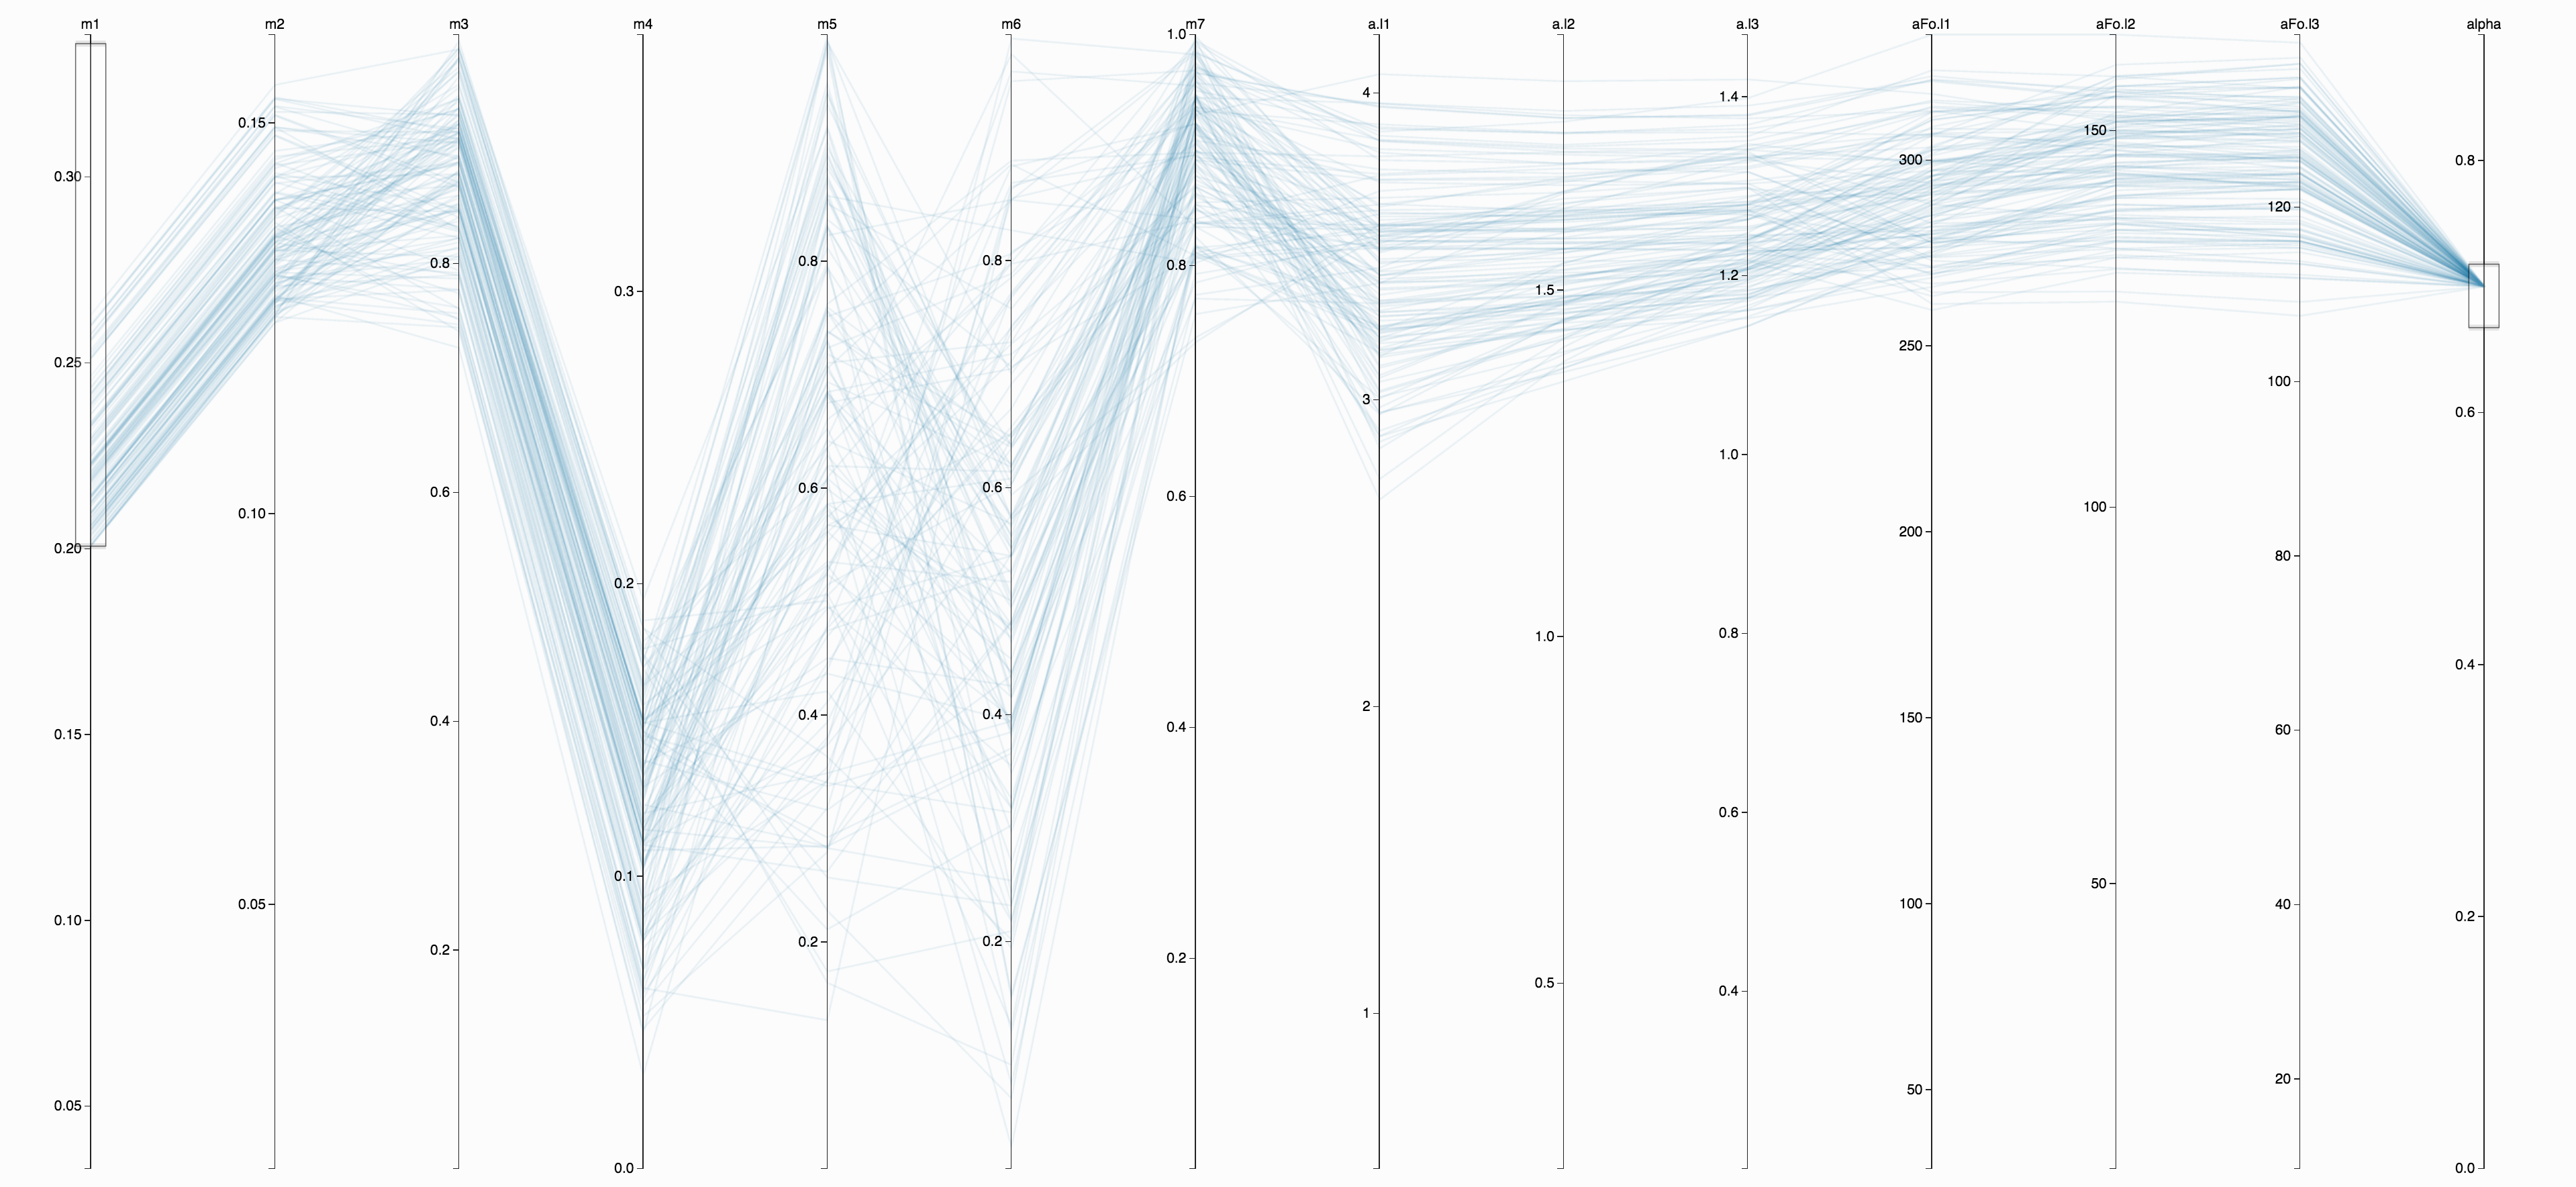
\includegraphics[width=1.0\textwidth]{figs/X_a8_upper.png}
  \end{center}
  \caption{Upper for Muscle 1}
  \label{fig_high}
\end{figure}

\begin{figure}[ht]
   \begin{center}
    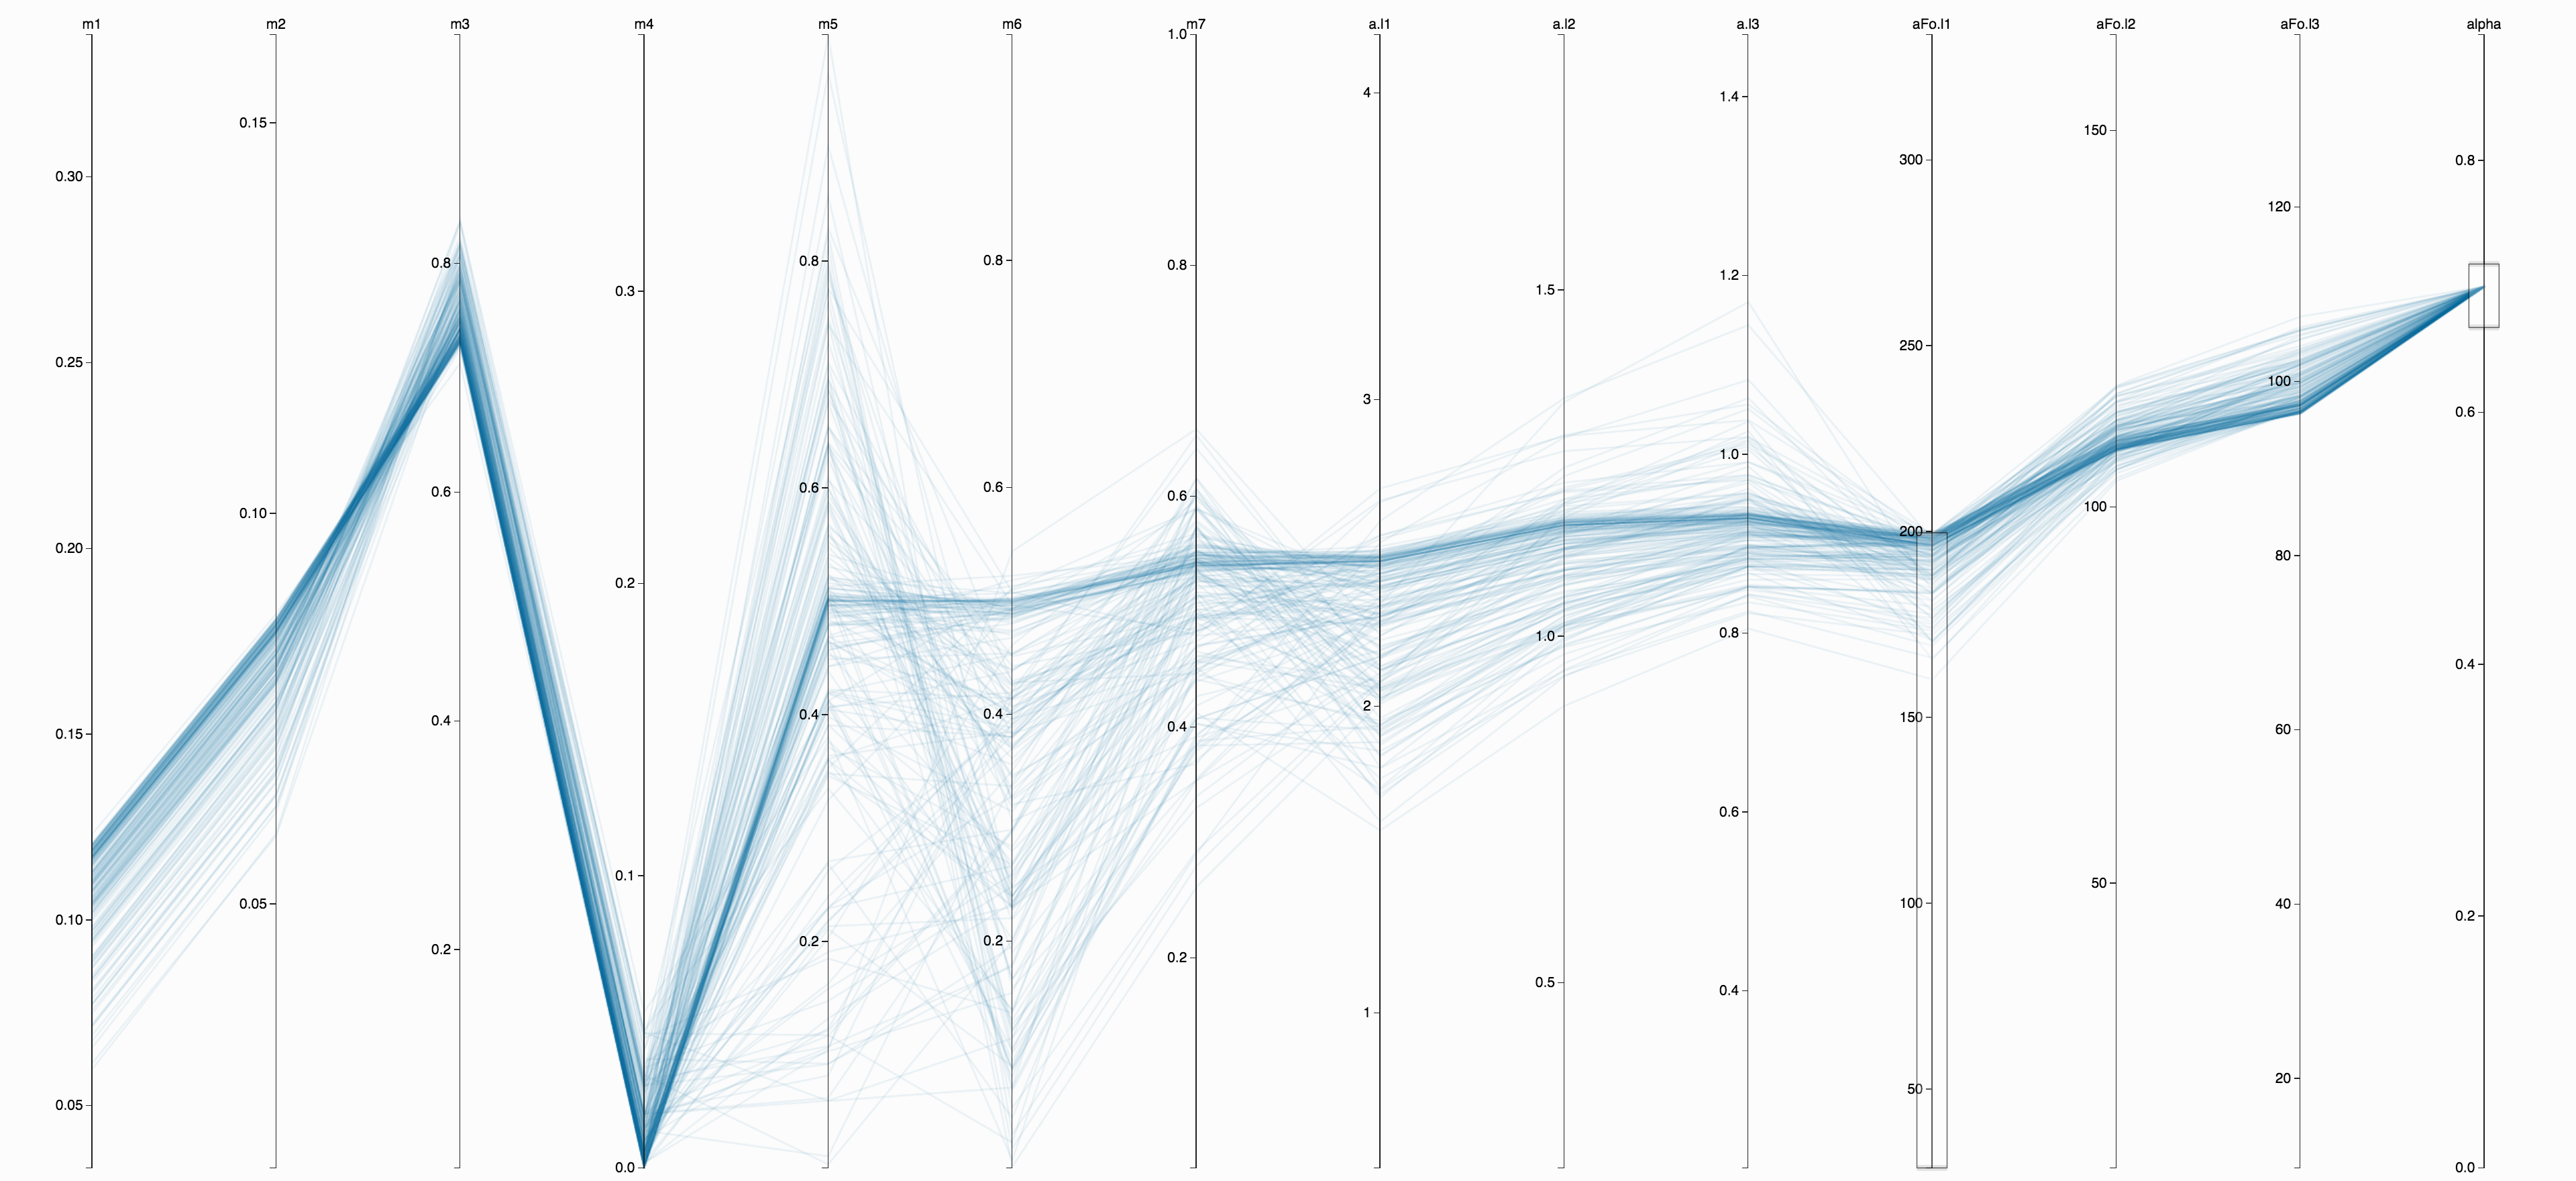
\includegraphics[width=1.0\textwidth]{figs/X_a8_weightedcost.png}
  \end{center}
  \caption{Weighted Cost}
  \label{fig_cost}
\end{figure}

\textit{Muscle 5 and 6 same direction and same strength $\Rightarrow$ Does not matter which one we activate for low cost}
